\section{Виды ошибок}
\subsection{Неправильное внесение сумм (ошибки ввода)}
\marginnote{\Date{Пт.}{13}{Июл.}{2018}}[-40pt]

\begin{itemize}	
	\item Одной из самых распространненых ошибок является неправильный ввод сумм. Когда путают местами цифры в числе, забывают проставить копейки или вносят неправильные значения.
	\\
	\\
	\begin{figure}[H]
		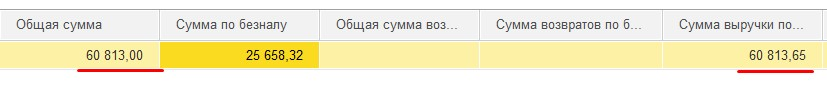
\includegraphics[width=1.0\textwidth]{5.jpg}
		\caption{Неправильный ввод.}
		\label{ris:5.jpg}
	\end{figure}
	В данном случае кассир не внес 65 коп. в поле <<Общая сумма>> (Рис.~\ref{ris:5.jpg})	
	\\
	\\	
	\begin{figure}[H]
		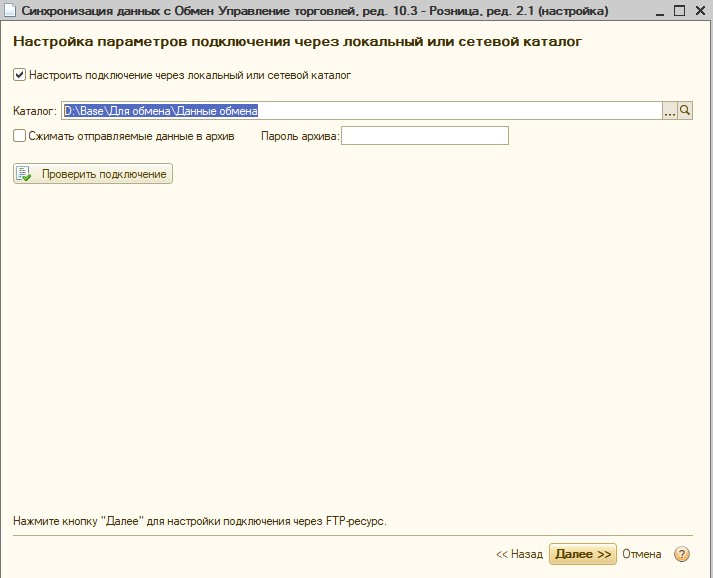
\includegraphics[width=1.0\textwidth]{6.jpg}
		\caption{Отсутствие значений.}
		\label{ris:6.jpg}
	\end{figure}
	Здесь не была внесена сумма по эквайрингу не смотря на наличие безнальных платежей.  (Рис.~\ref{ris:6.jpg})	
	\\
	\\
		\begin{figure}[H]
		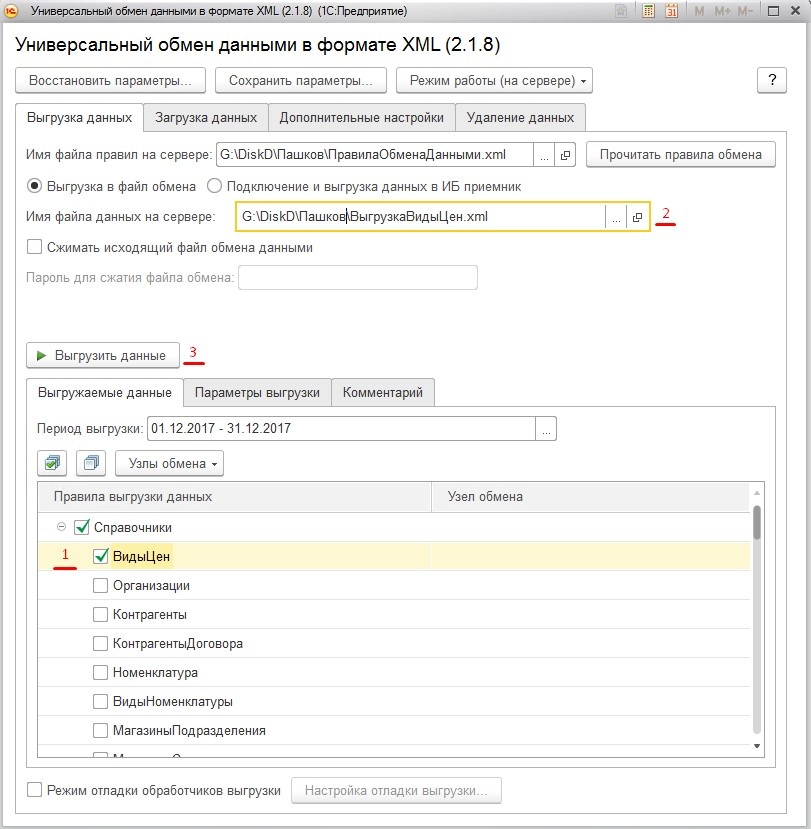
\includegraphics[width=1.0\textwidth]{7.jpg}
		\caption{Изменен порядок цифр в числе.}
		\label{ris:7.jpg}
	\end{figure}
	Здесь  перепутаны местами цифры <<Общей суммы>> и <<Суммы выручки по ОРП>>.  (Рис.~\ref{ris:7.jpg})	
	
	\newpage
	\item Для исправления этих ошибок дважды кликаем мышкой на строке с ошибками. Появляется окно редактирования  (Рис.~\ref{ris:7.jpg})	
			\begin{figure}[H]
		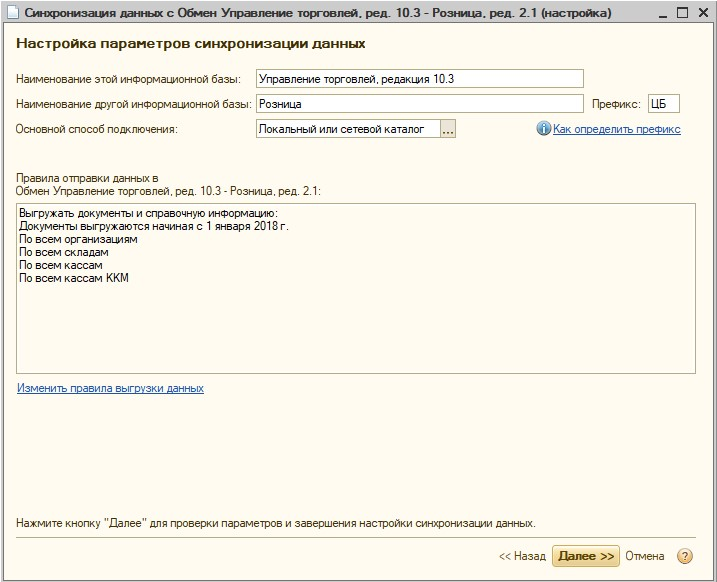
\includegraphics[width=0.6\textwidth]{8.jpg}
		\caption{Окно редактирования.}
		\label{ris:8.jpg}
	\end{figure}
	
	Сверяясь с бумажнвми документами заносим суммы в соответствующие поля. По окончании нажимаем \keys{Записать и закрыть}.
	Появляется новая строка с исправленными данными. Пробуем провести документ  ОРП. Если данные корректны, то документ проведется.
	Через меню <<Связанные документы>> (Рис.~\ref{ris:9.jpg})  переходим к <<Акту списания ЕГАИС>>.

		
	\begin{figure}[H]
		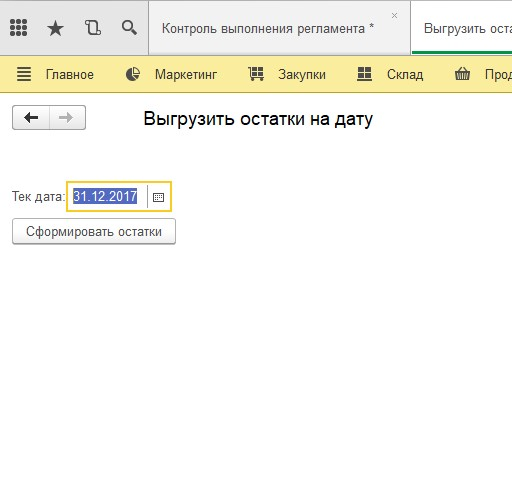
\includegraphics[width=0.6\textwidth]{9.jpg}
		\caption{Связанные документы.}
		\label{ris:9.jpg}
	\end{figure}
	
	\newpage
	 Проводим его и отправляем в ЕГАИС. (Рис.~\ref{ris:10.jpg})
	 
	 	\begin{figure}[H]
	 	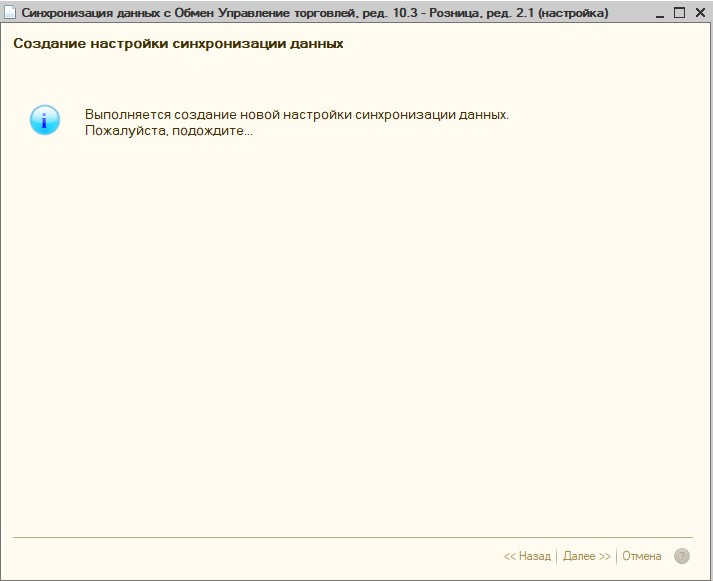
\includegraphics[width=0.9\textwidth]{10.jpg}
	 	\caption{Акт списания ЕГАИС.}
	 	\label{ris:10.jpg}
	 \end{figure}
	 
	
	\todo{Расписать работы с актом списания}\par
	
\end{itemize}
